\chapter{Manual de usuario}

\section{Instalación}

Para poder instalar la aplicación será necesario disponer de una versión de Android igual o superior a la versión 4.4 de Android, puesto que necesitamos compatibilidad con Android Wear. Se debe además disponer de un dispositivo que utilice Android Wear 1.0 o superior.\\
\\
\subsection*{Móvil}
Para instalar la aplicación en un terminal se debe transferir a dicho terminal el archivo apk. Una vez se encuentra en el dispositivo, se debe habilitar la instalación desde origenes desconocidos. Para ello se deberá acceder a la opción de ajustes/seguridad y activar la opción de aplicaciones de origen desconocido.

\begin{figure}[H]
	\centering
	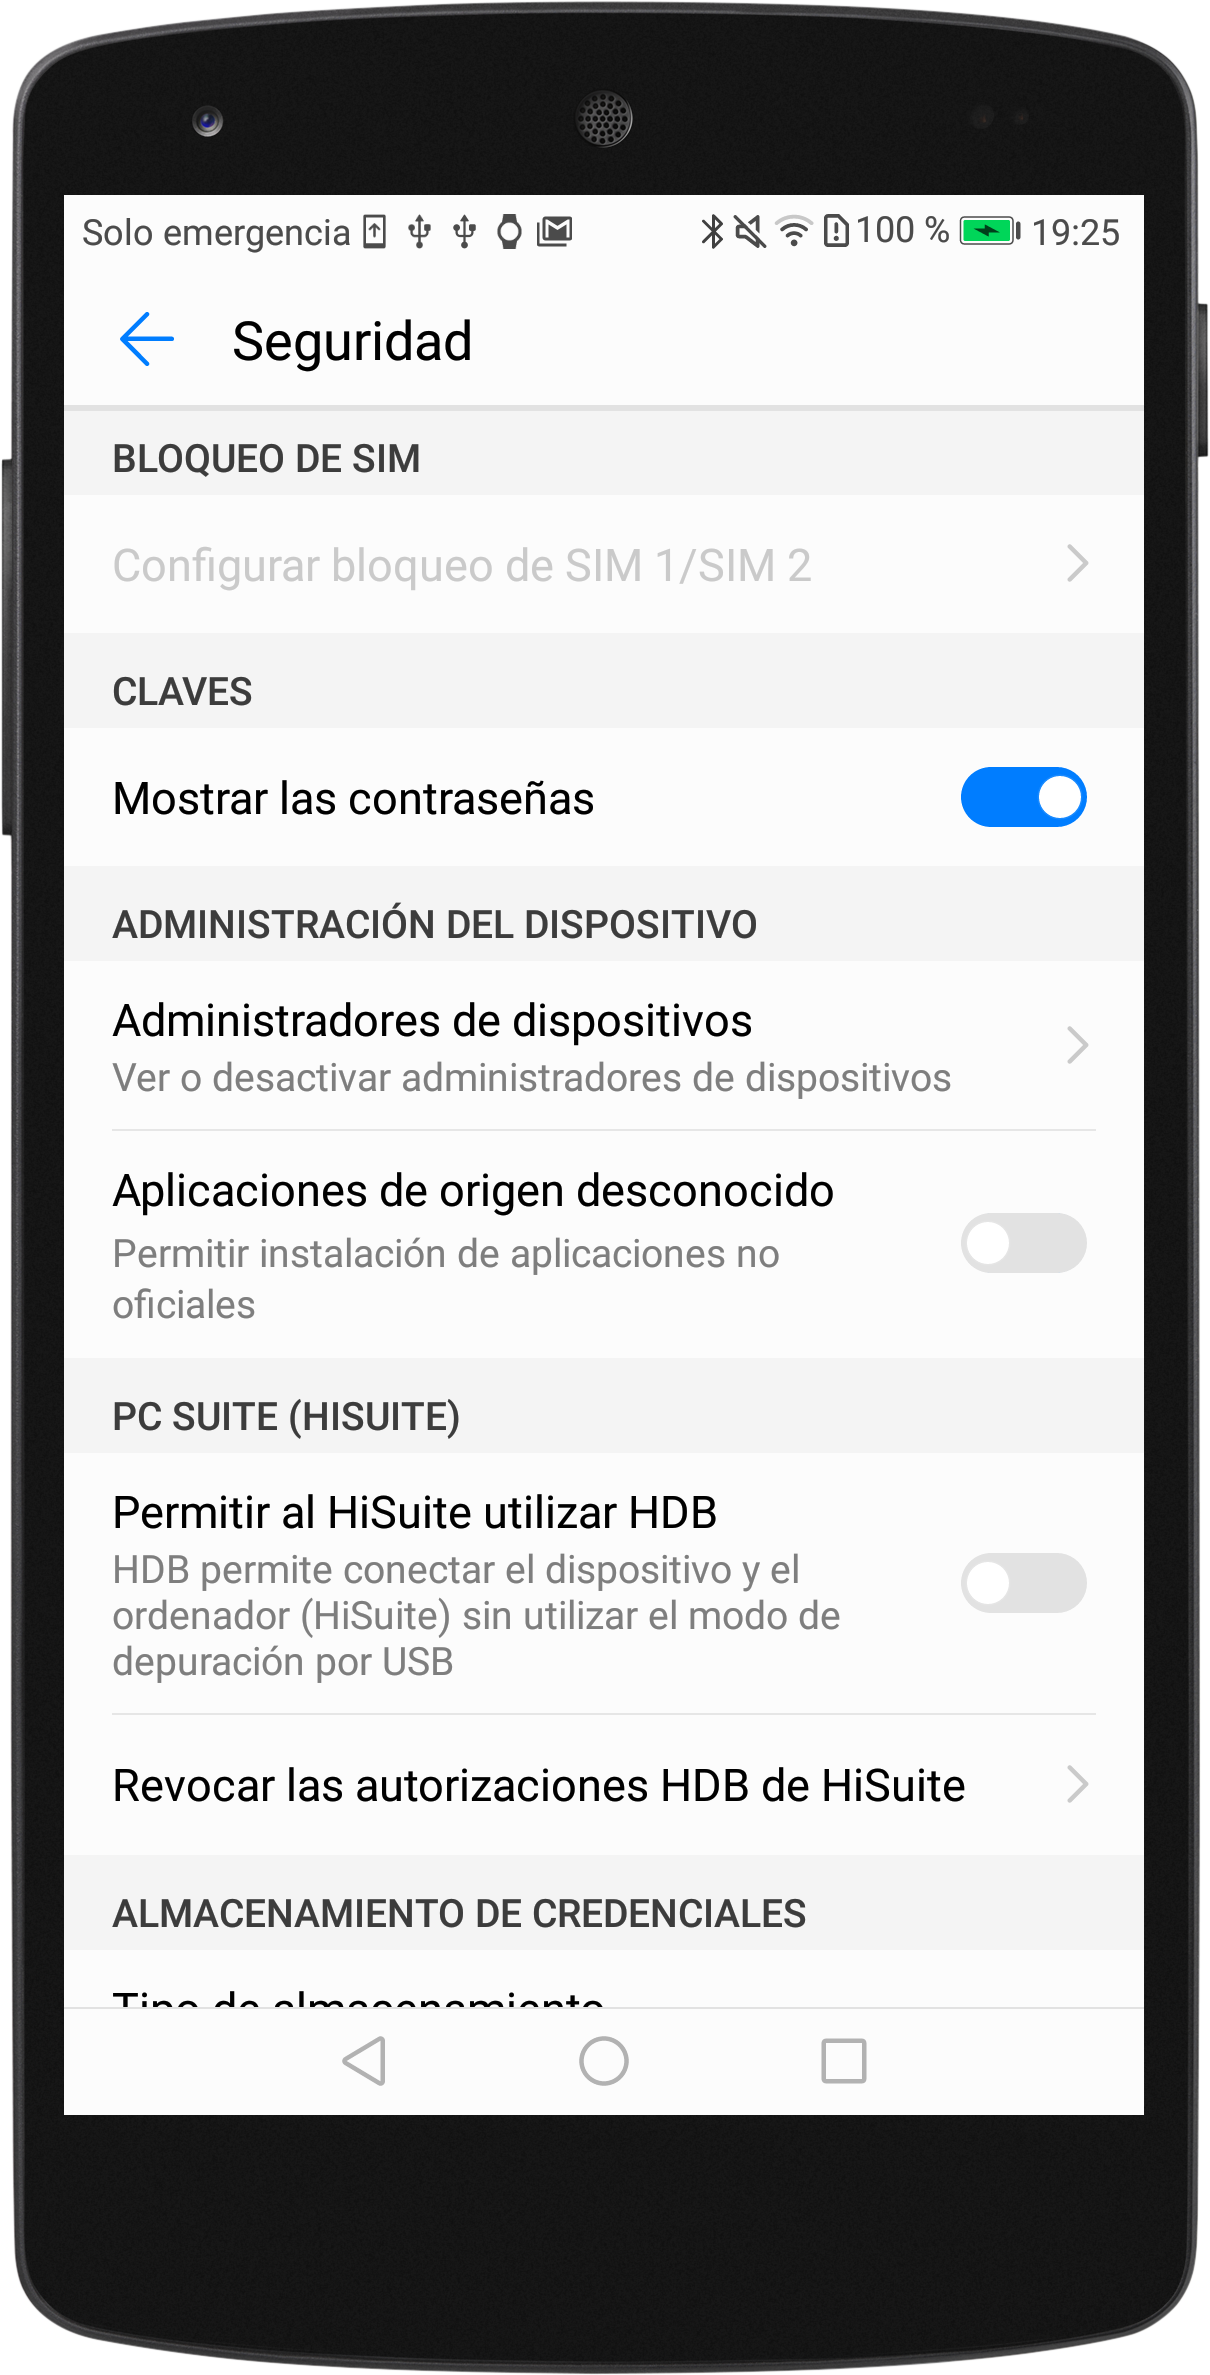
\includegraphics[scale=0.17]{imagenes/seguridad.png}
	\caption{Instalación desde origen desconocido.}
	\label{Instalación desde origen desconocido}
\end{figure}

Una vez esta la opción habilitada, simplemente se tendrá que seleccionar el apk desde el explorador de archivos por defecto y se procederá a su instalación.

\subsection*{Wear}

Para instalar la aplicación en el dispositivo wearable, se deberá activar las opciones de desarrollador del dispositivo, para ello se debe acceder a la opcion de información y seleccionando repetidas veces sobre el número de compilación se podrá acceder a las opciones de desarrollador. Una vez activadas las opciones de desarrollador se deberá permitir la depuración en el dispositivo.


\begin{figure}[H]
	\centering
	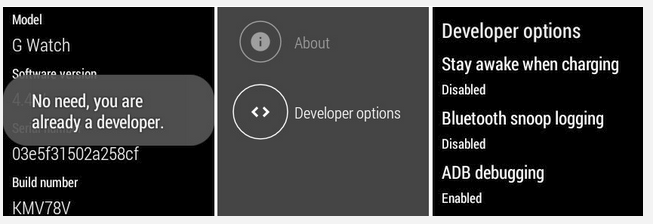
\includegraphics[scale=0.5]{imagenes/dev.png}
	\caption{Modo depuración Android Wear \cite{depur}.}
	\label{Modo depuración Android Wear}
\end{figure}

Con el archivo apk en el ordenador y en el directorio actual, solo quedará ejecutar en un terminal:
\\
\\
\$adb forward tcp:4444 localabstract:/adb–hub \\
\$adb connect localhost:4444 \\
\$adb -e install app.apk \\

\section{Creación de usuario}

Para crear un usuario simplemente se debe abrir la aplicación, hacer click en Registro y rellenar los credenciales necesarios.


\begin{figure}[H]
	\centering
	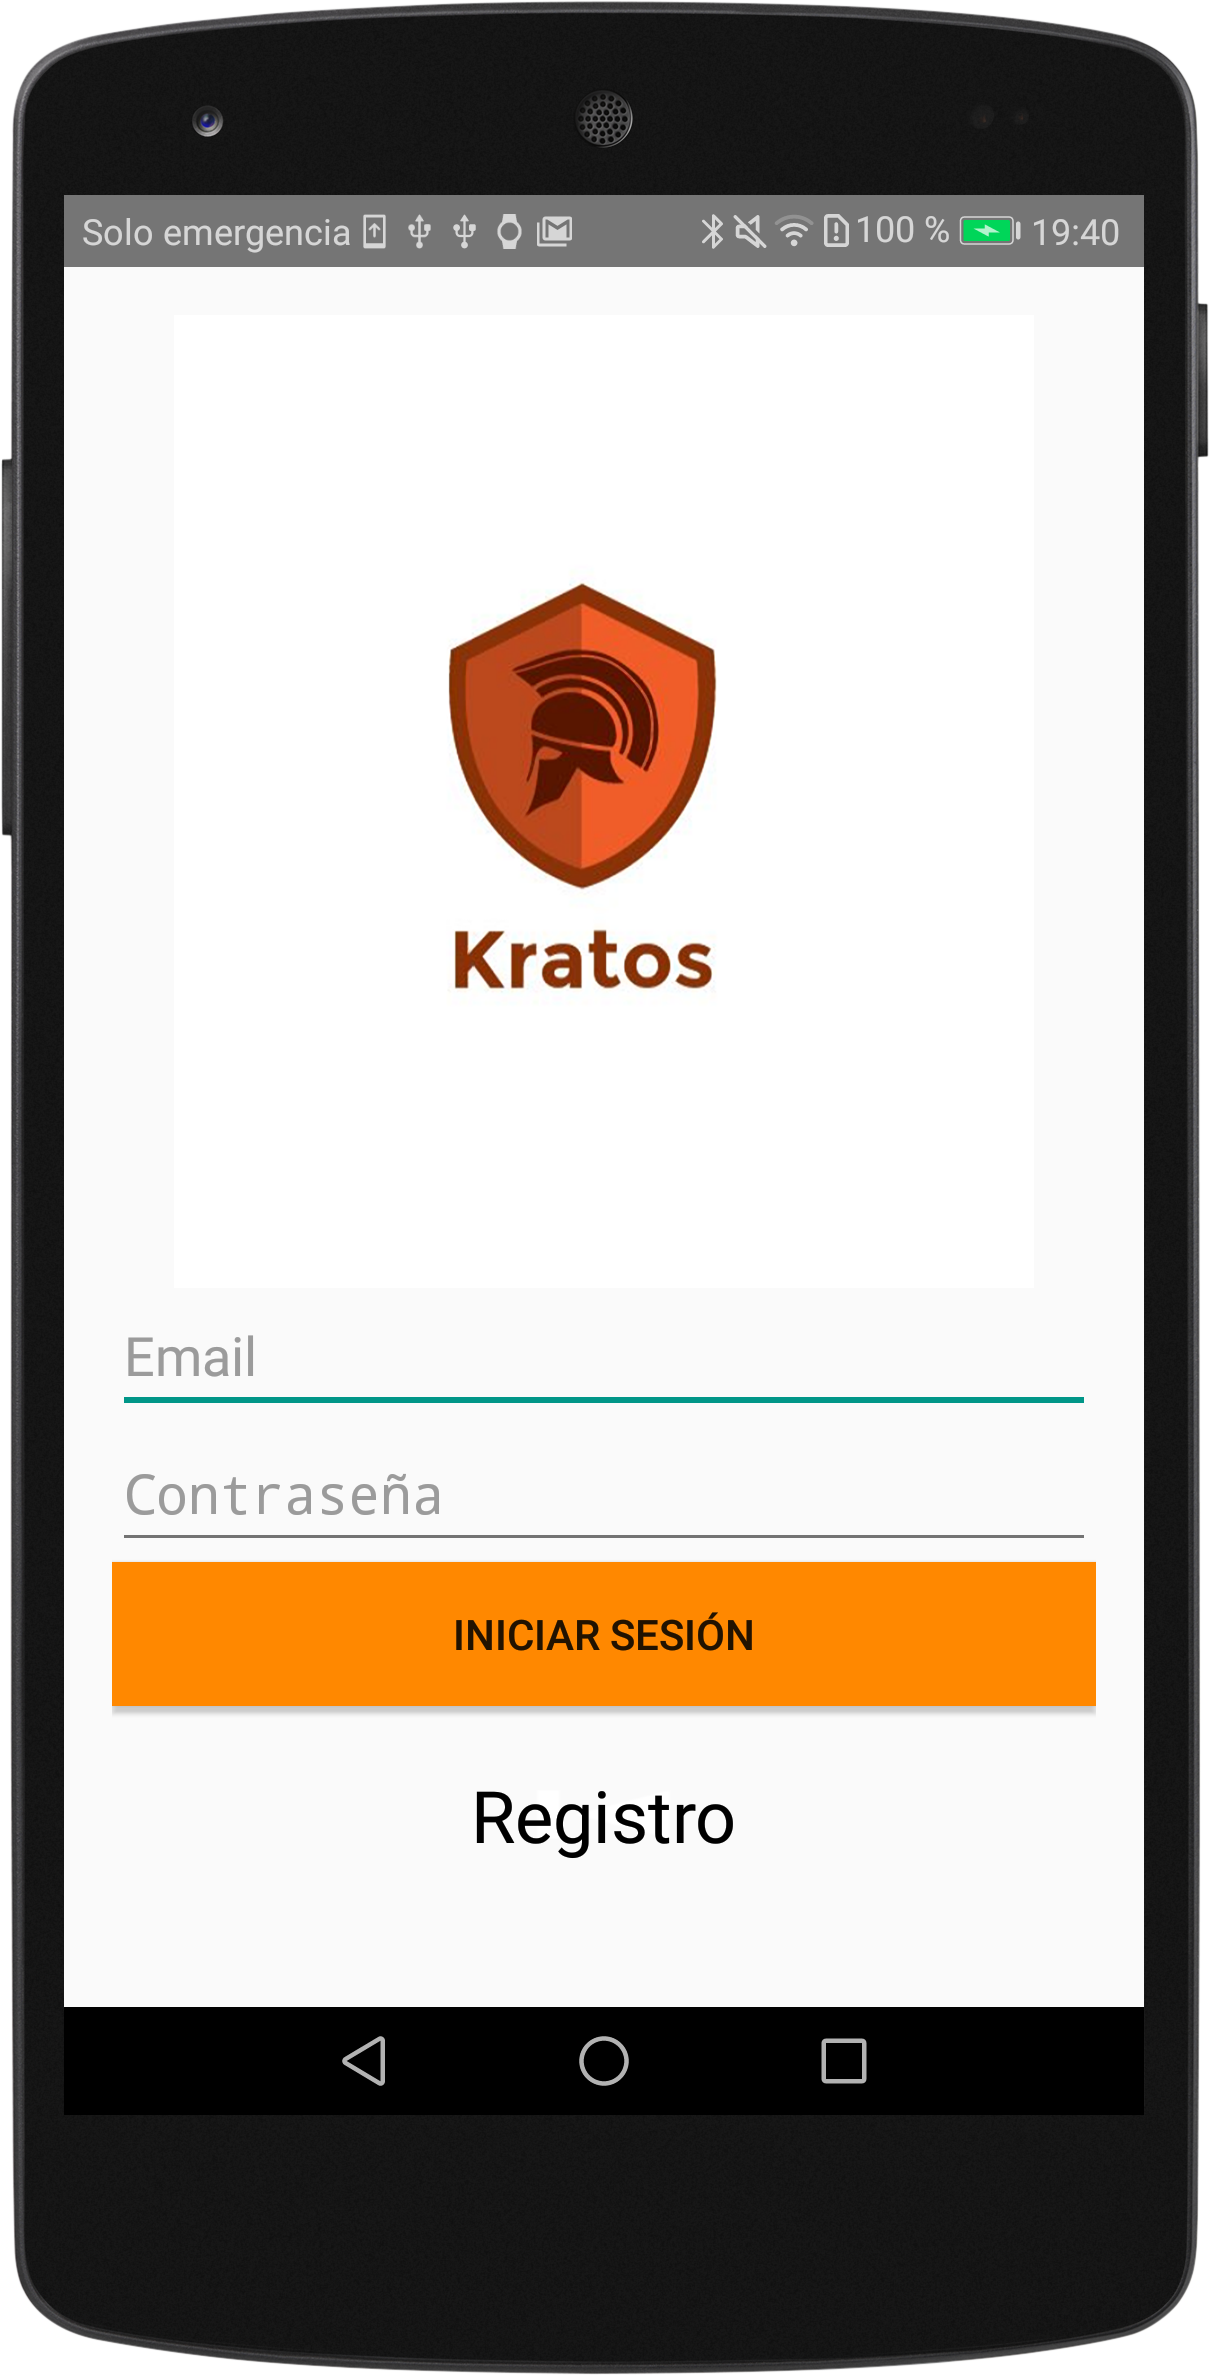
\includegraphics[scale=0.10]{imagenes/m1.png}
	\caption{Regristro 1.}
	\label{Regristro 1}
\end{figure}

\begin{figure}[H]
	\centering
	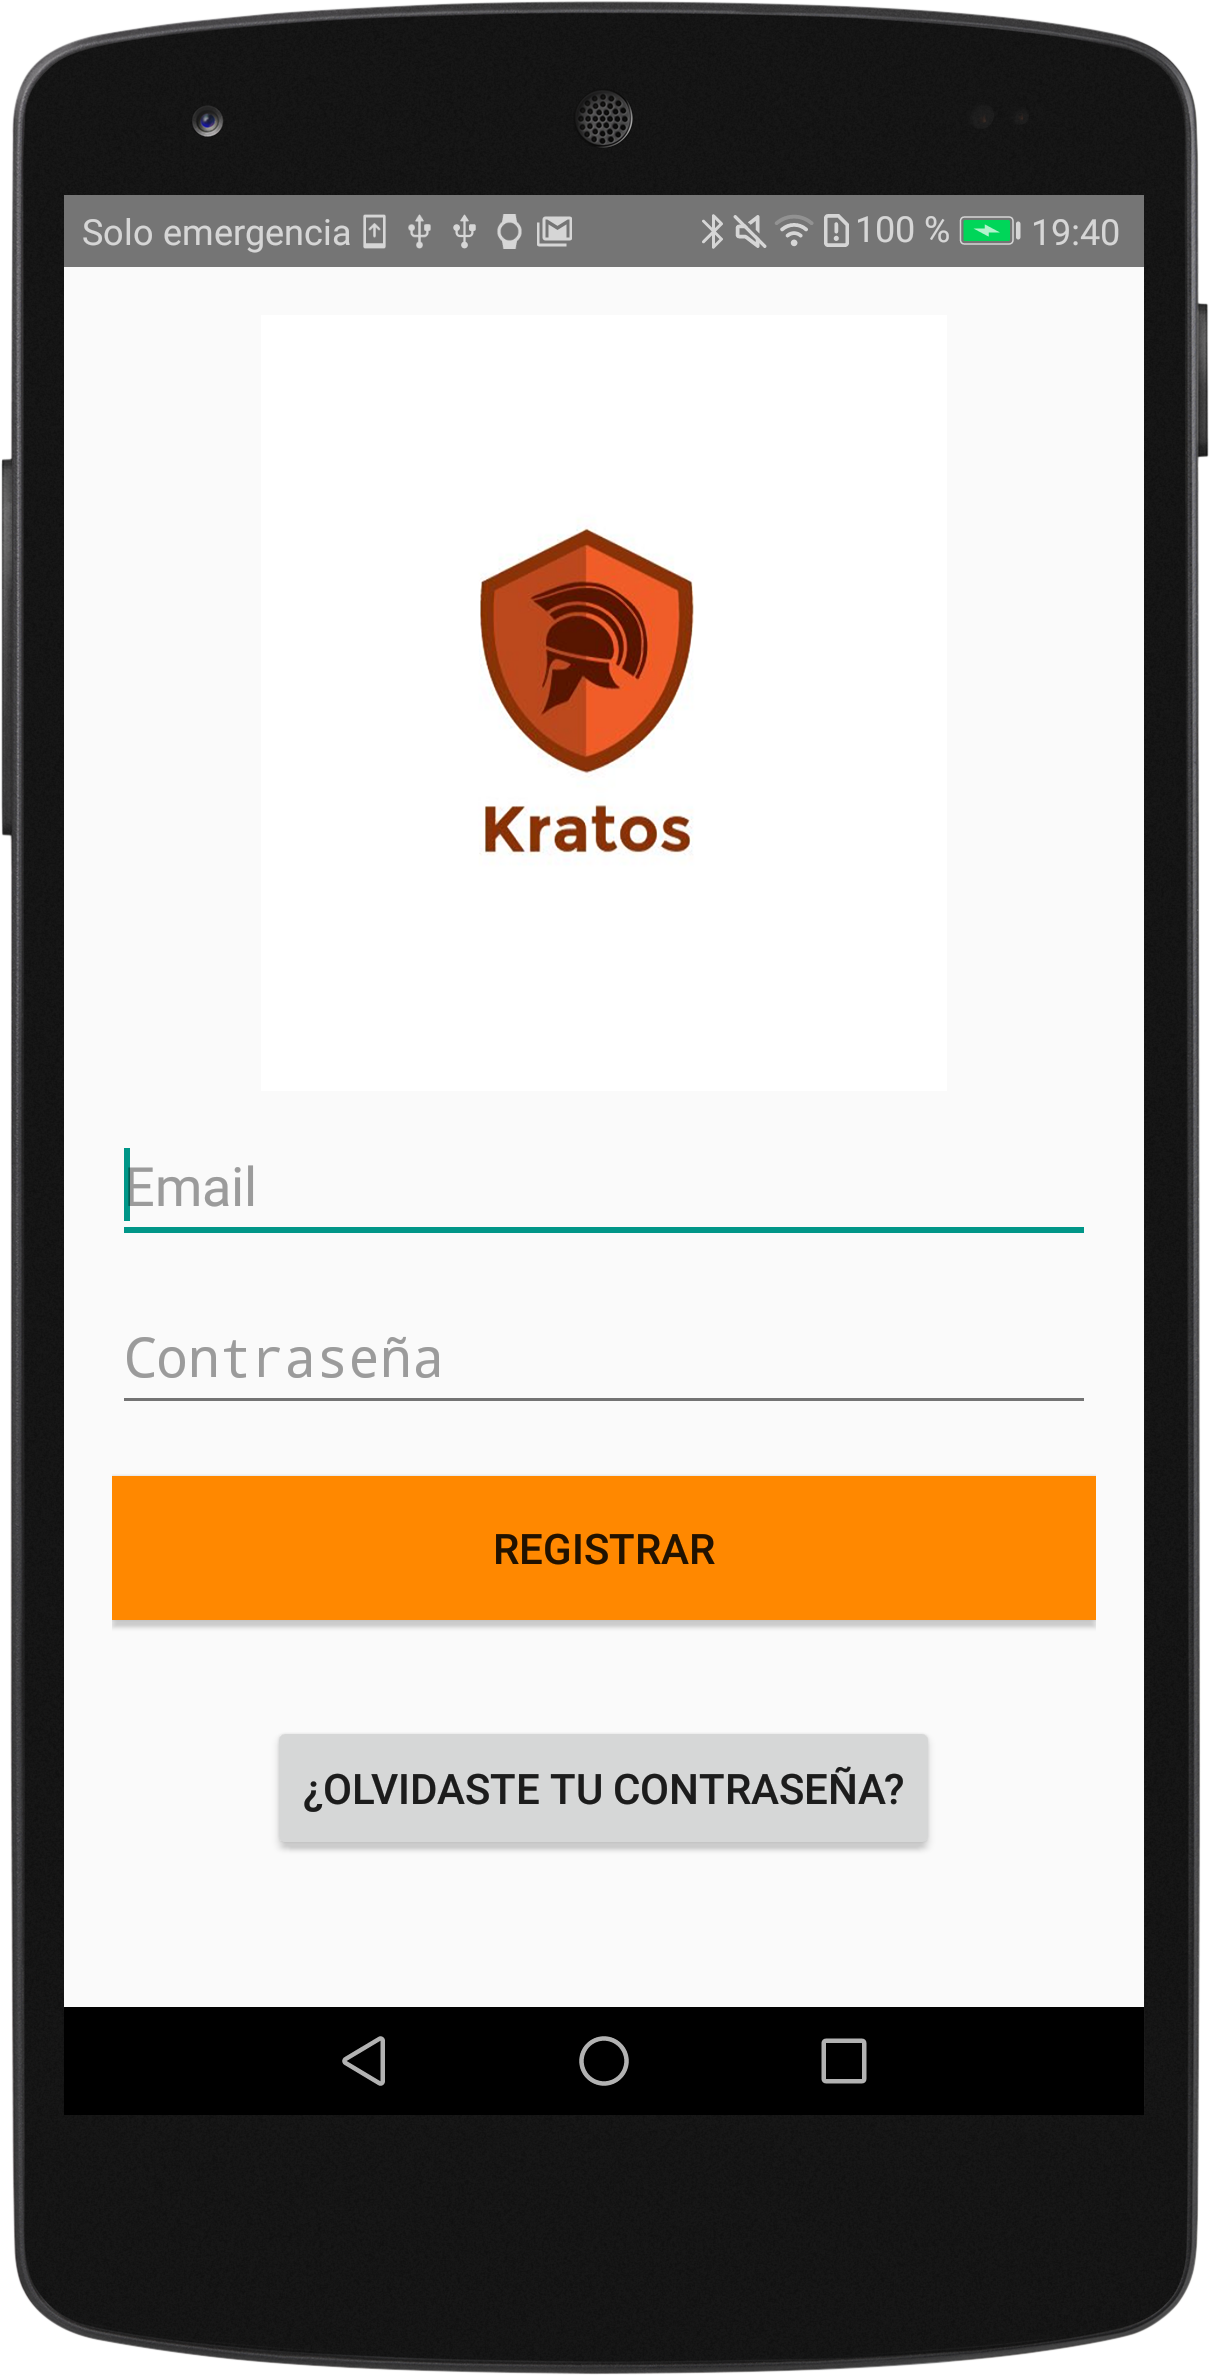
\includegraphics[scale=0.11]{imagenes/registro.png}
	\caption{Regristro 2.}
	\label{Regristro 2}
\end{figure}

\section{Realización ejercicio}

Para realizar la monitorización del ejercicio se debe seleccionar la pestaña ejercicio, seleccionar el ejercicio deseado y empezar el ejercicio. De manera paralela una vez hayamos llegado a la Ejemplo de monitorización, activaremos la aplicación wear y se procederá a realizar el ejercicio.

\begin{figure}[H]
	\centering
	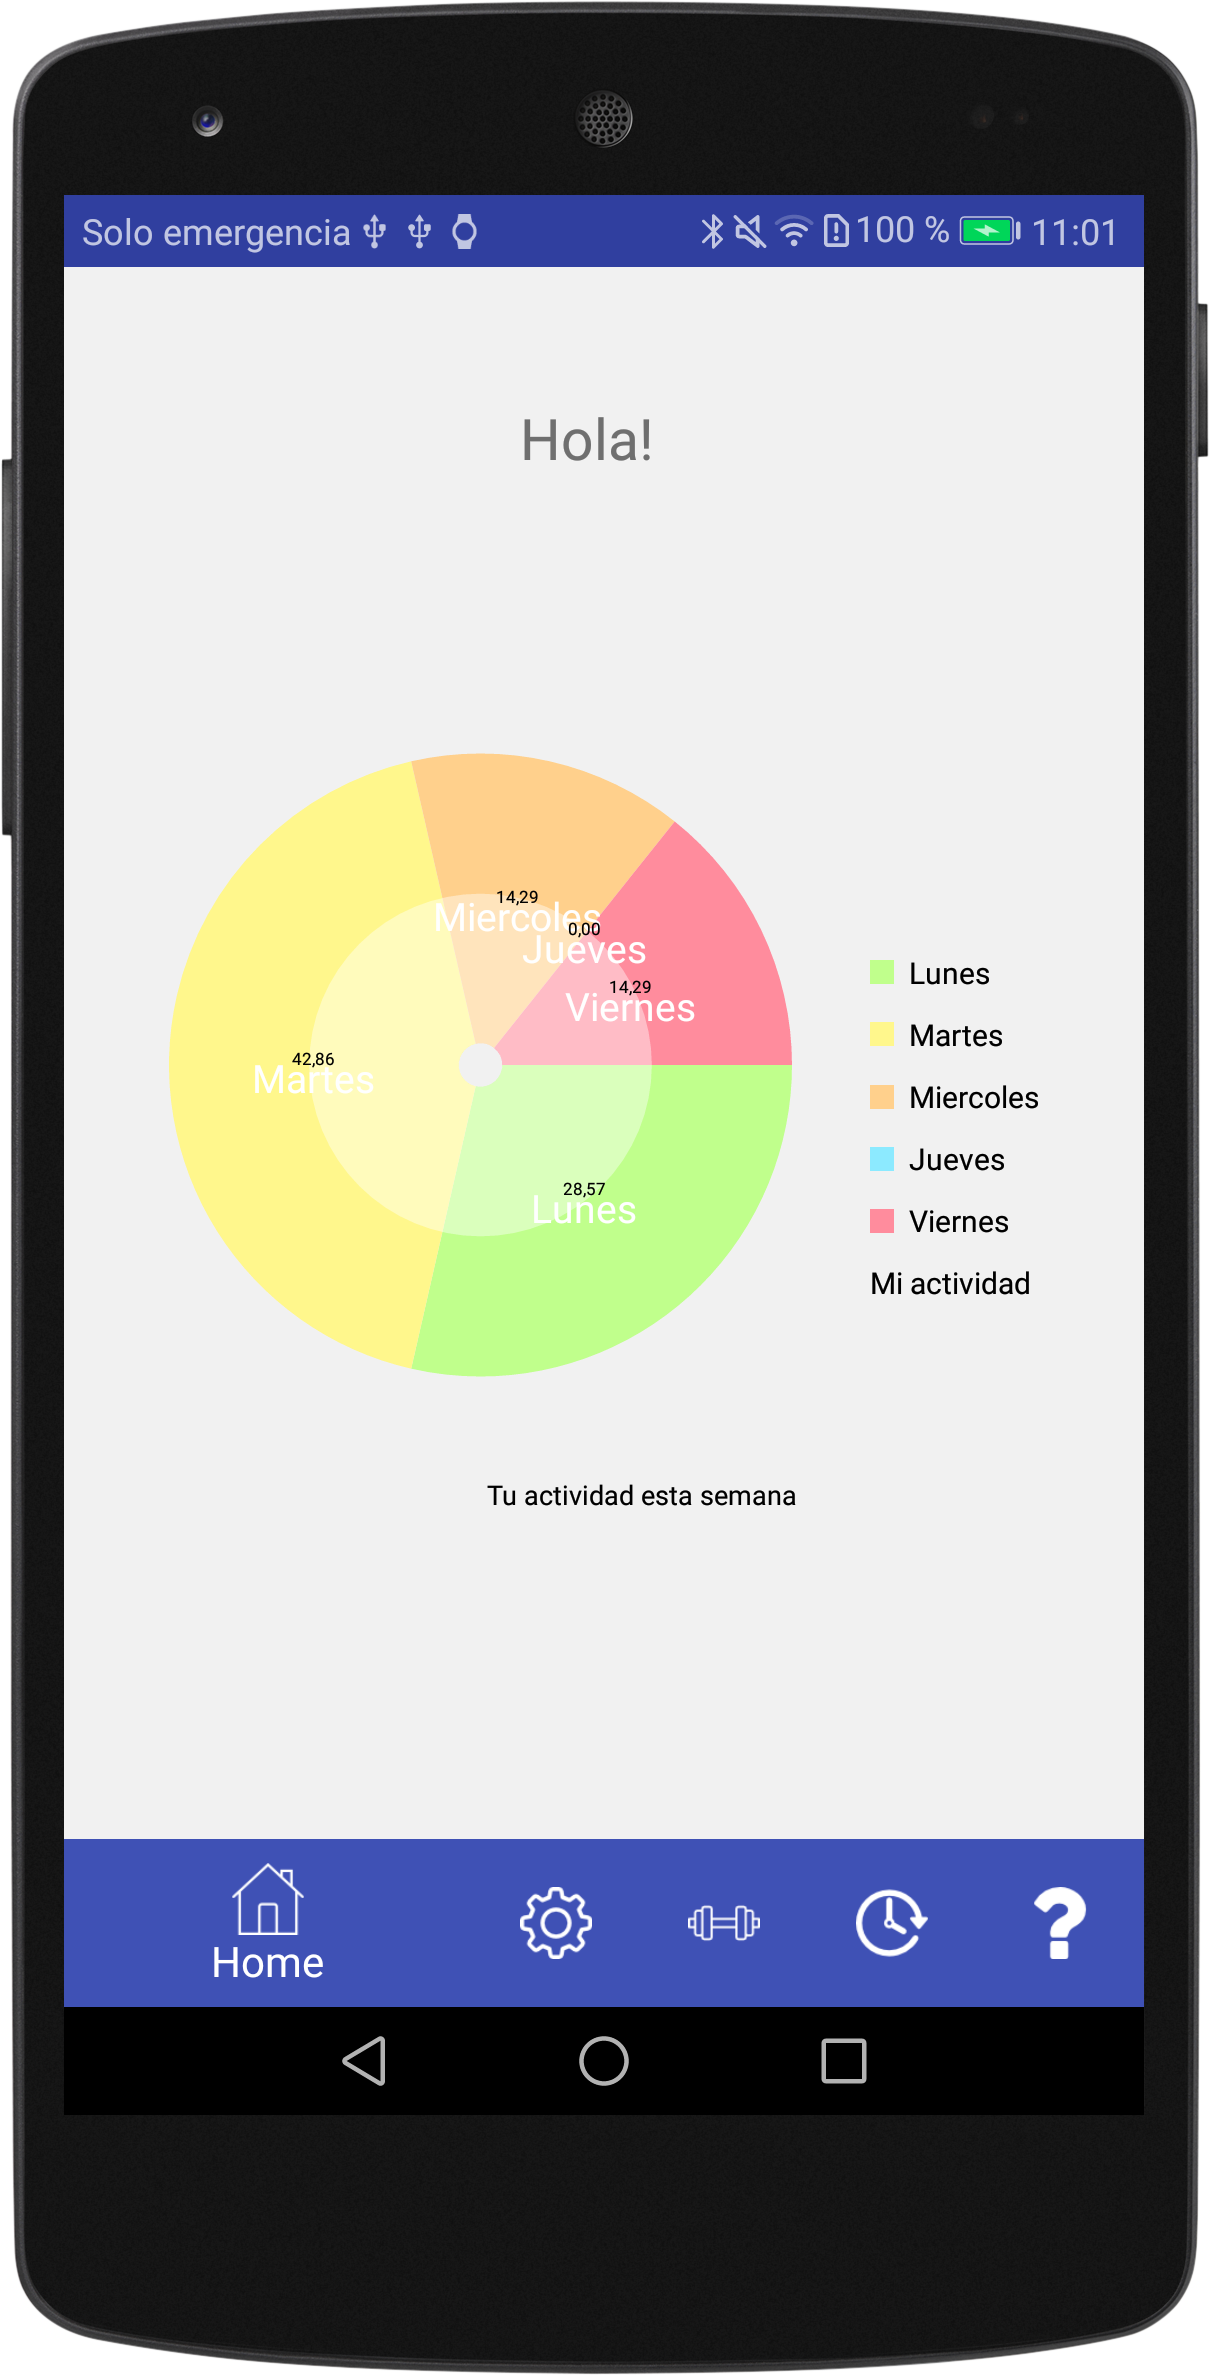
\includegraphics[scale=0.10]{imagenes/m2.png}
	\caption{Pantalla principal móvil}
	\label{Realización ejercicio 1}
\end{figure}


\begin{figure}[H]
	\centering
	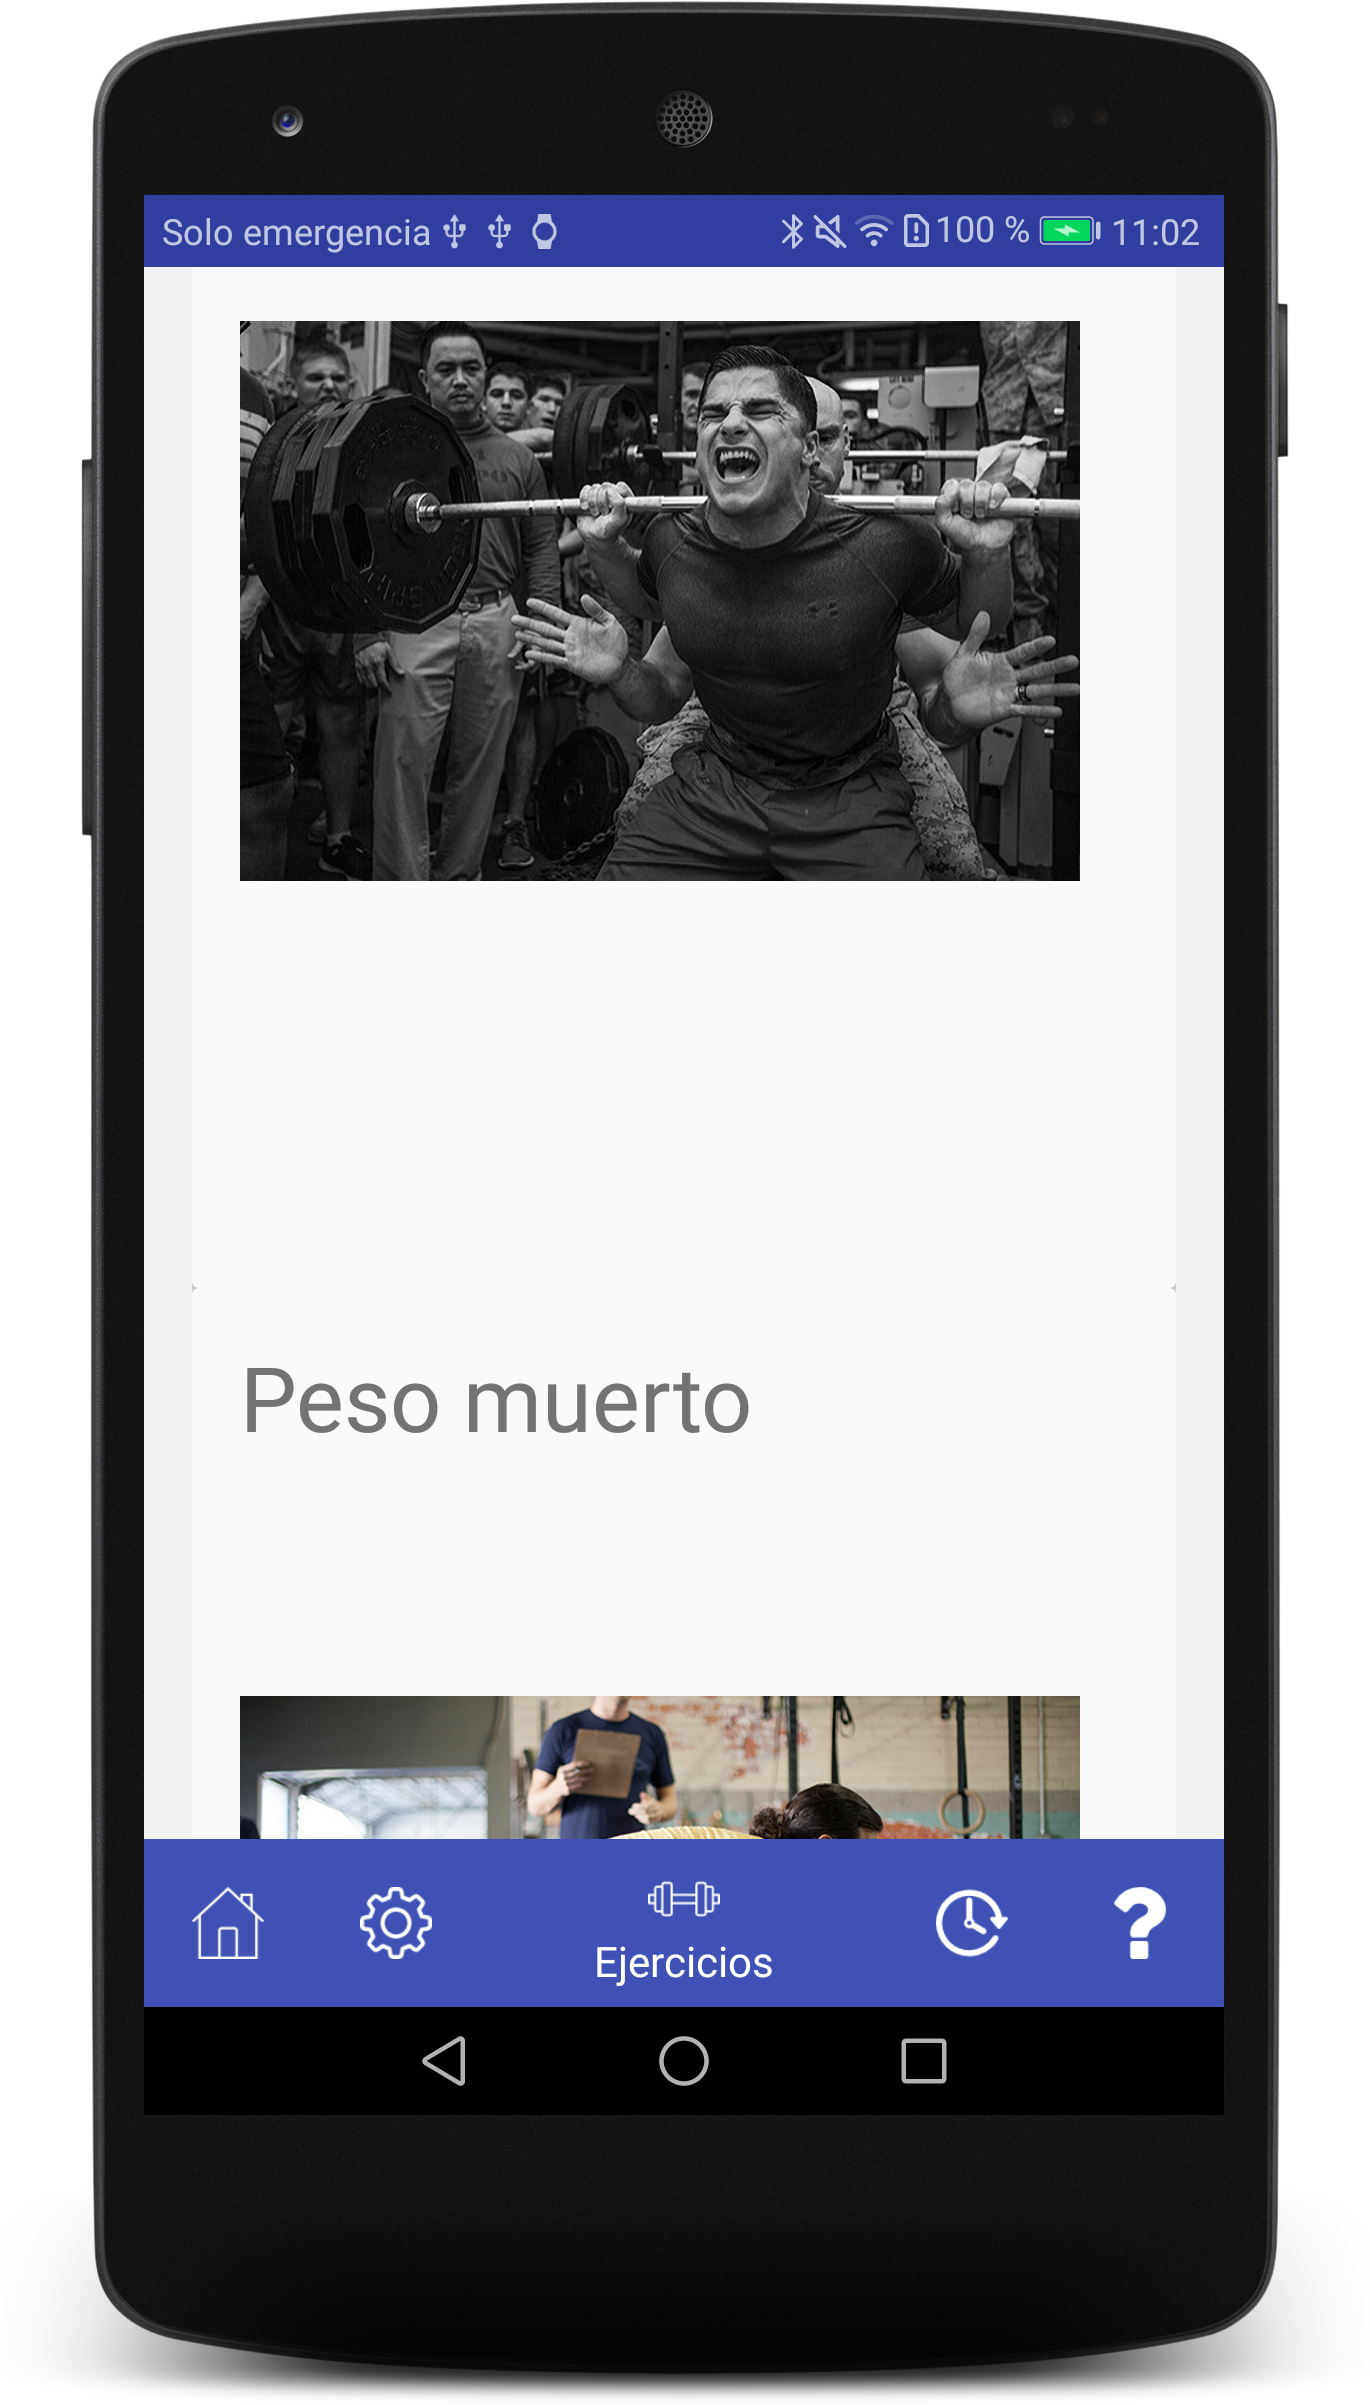
\includegraphics[scale=0.10]{imagenes/m4.png}
	\caption{Ejemplo selección ejercicio móvil}
	\label{Realización ejercicio 2}
\end{figure}

\begin{figure}[H]
	\centering
	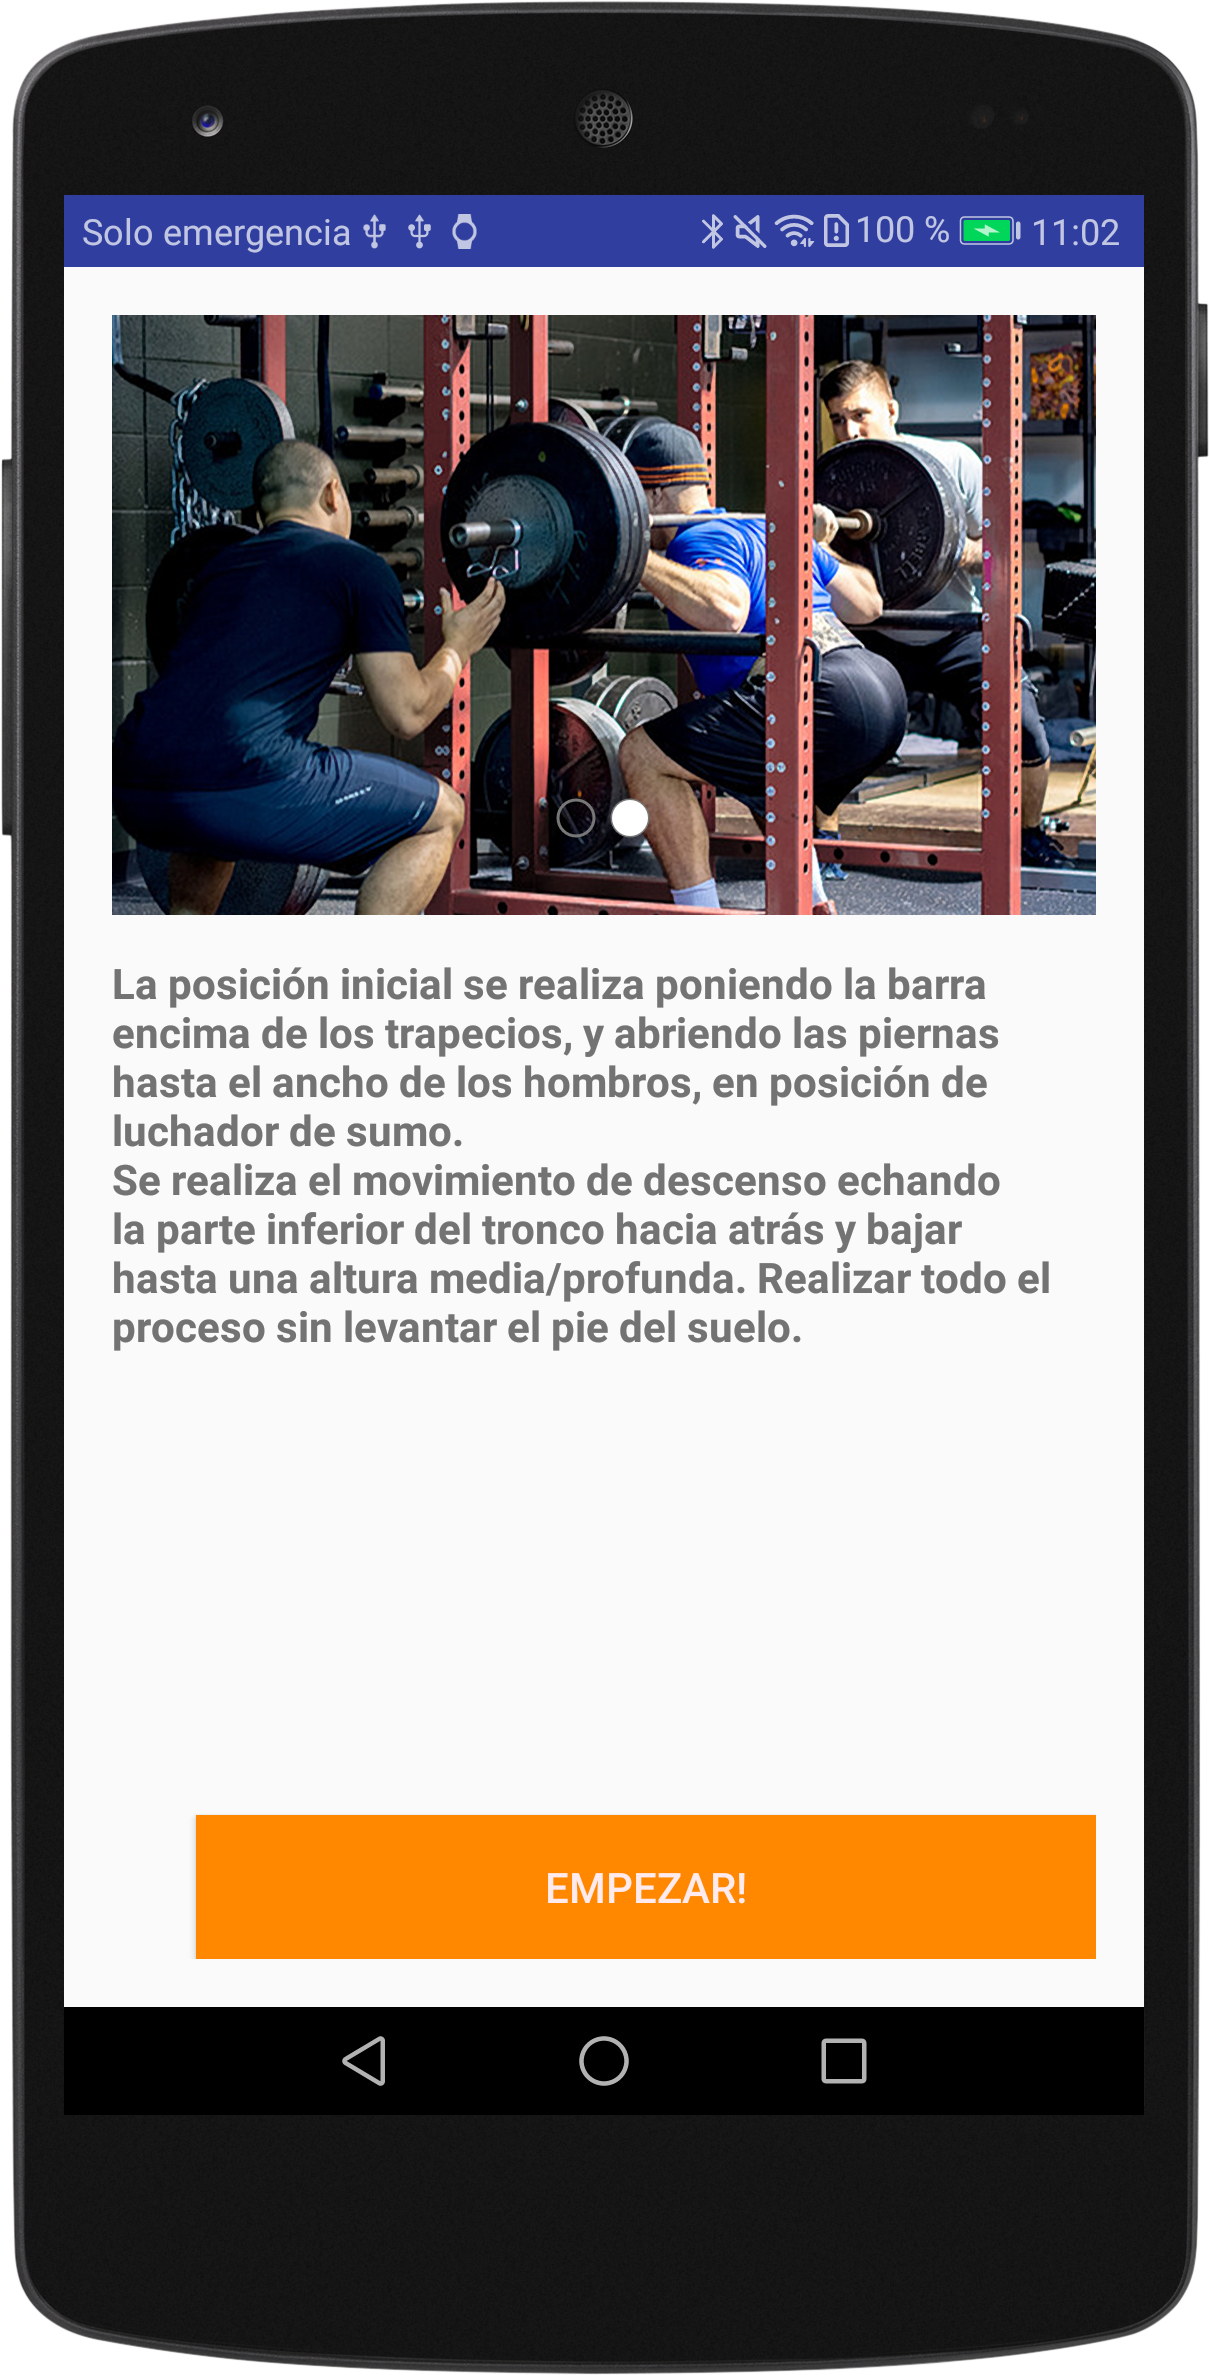
\includegraphics[scale=0.10]{imagenes/m5.png}
	\caption{Ejemplo descripción ejercicio móvil}
	\label{Realización ejercicio 3}
\end{figure}

\begin{figure}[H]
	\centering
	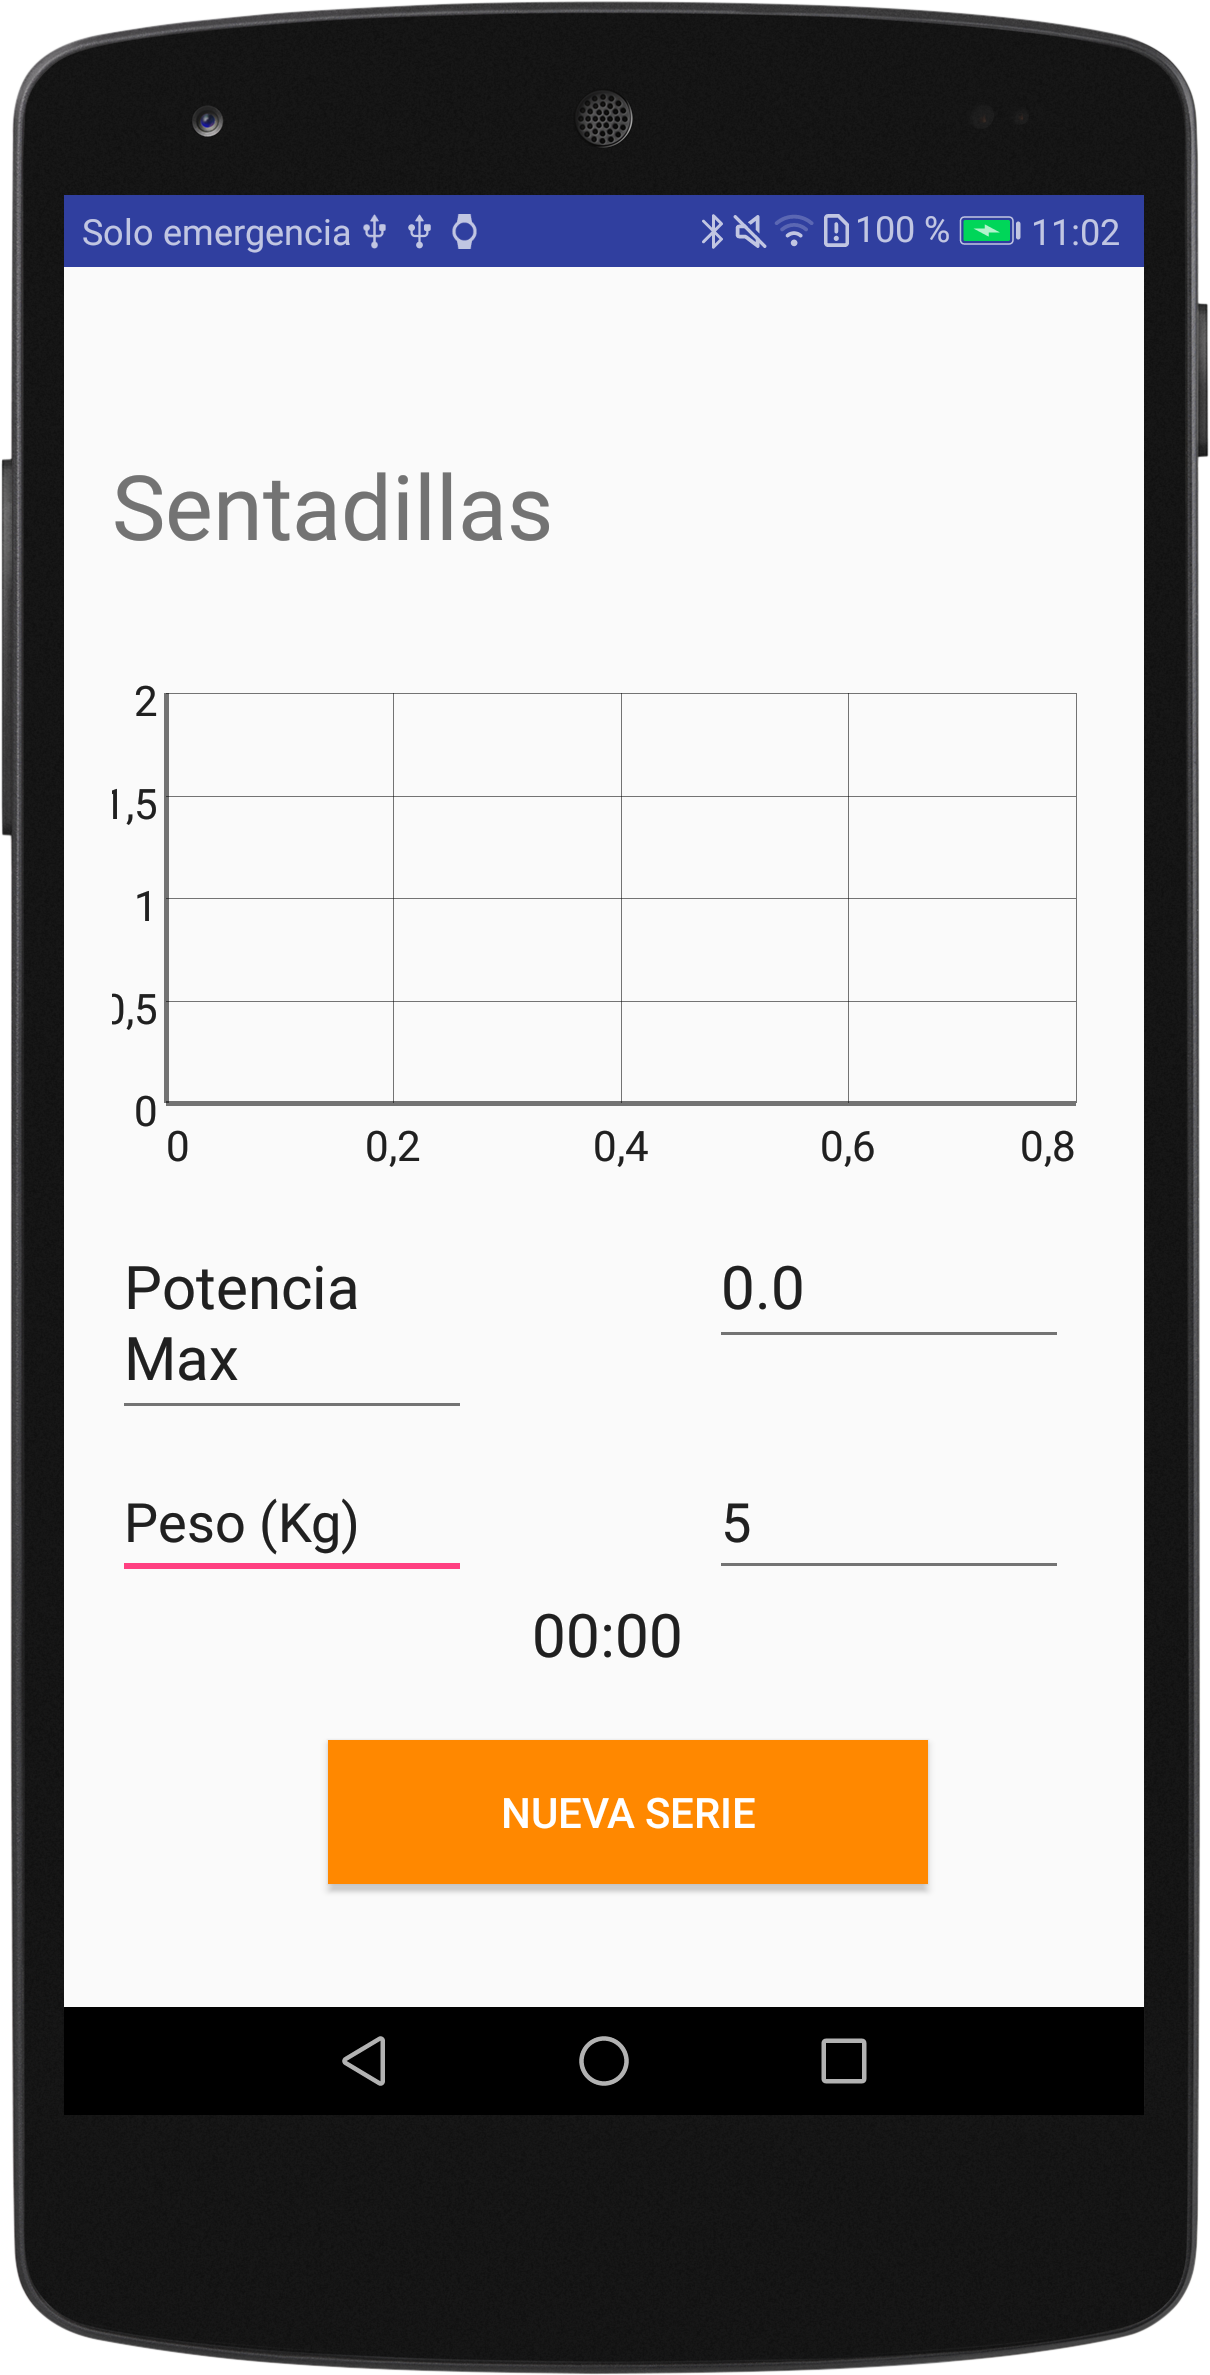
\includegraphics[scale=0.10]{imagenes/m6.png}
	\caption{Ejemplo iniciar ejercicio móvil}
	\label{Realización ejercicio 4}
\end{figure}

Se debe activar la aplicación wear e iniciar el ejercicio:

\begin{figure}[H]
	\centering
	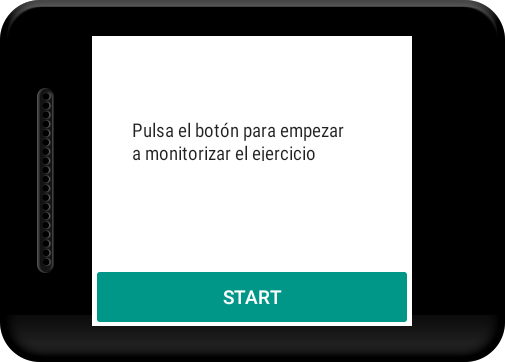
\includegraphics[scale=0.3]{imagenes/w1.png}
	\caption{Pantalla principal wear}
	\label{Realización ejercicio 5}
\end{figure}

\begin{figure}[H]
	\centering
	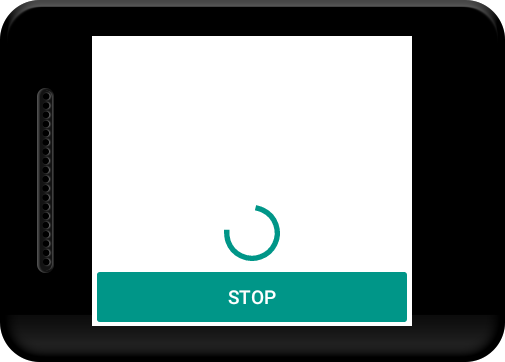
\includegraphics[scale=0.3]{imagenes/w2.png}
	\caption{Realizar medición wear}
	\label{Realización ejercicio 6}
\end{figure}


Finalmente monitorizando así el ejercicio

\begin{figure}[H]
	\centering
	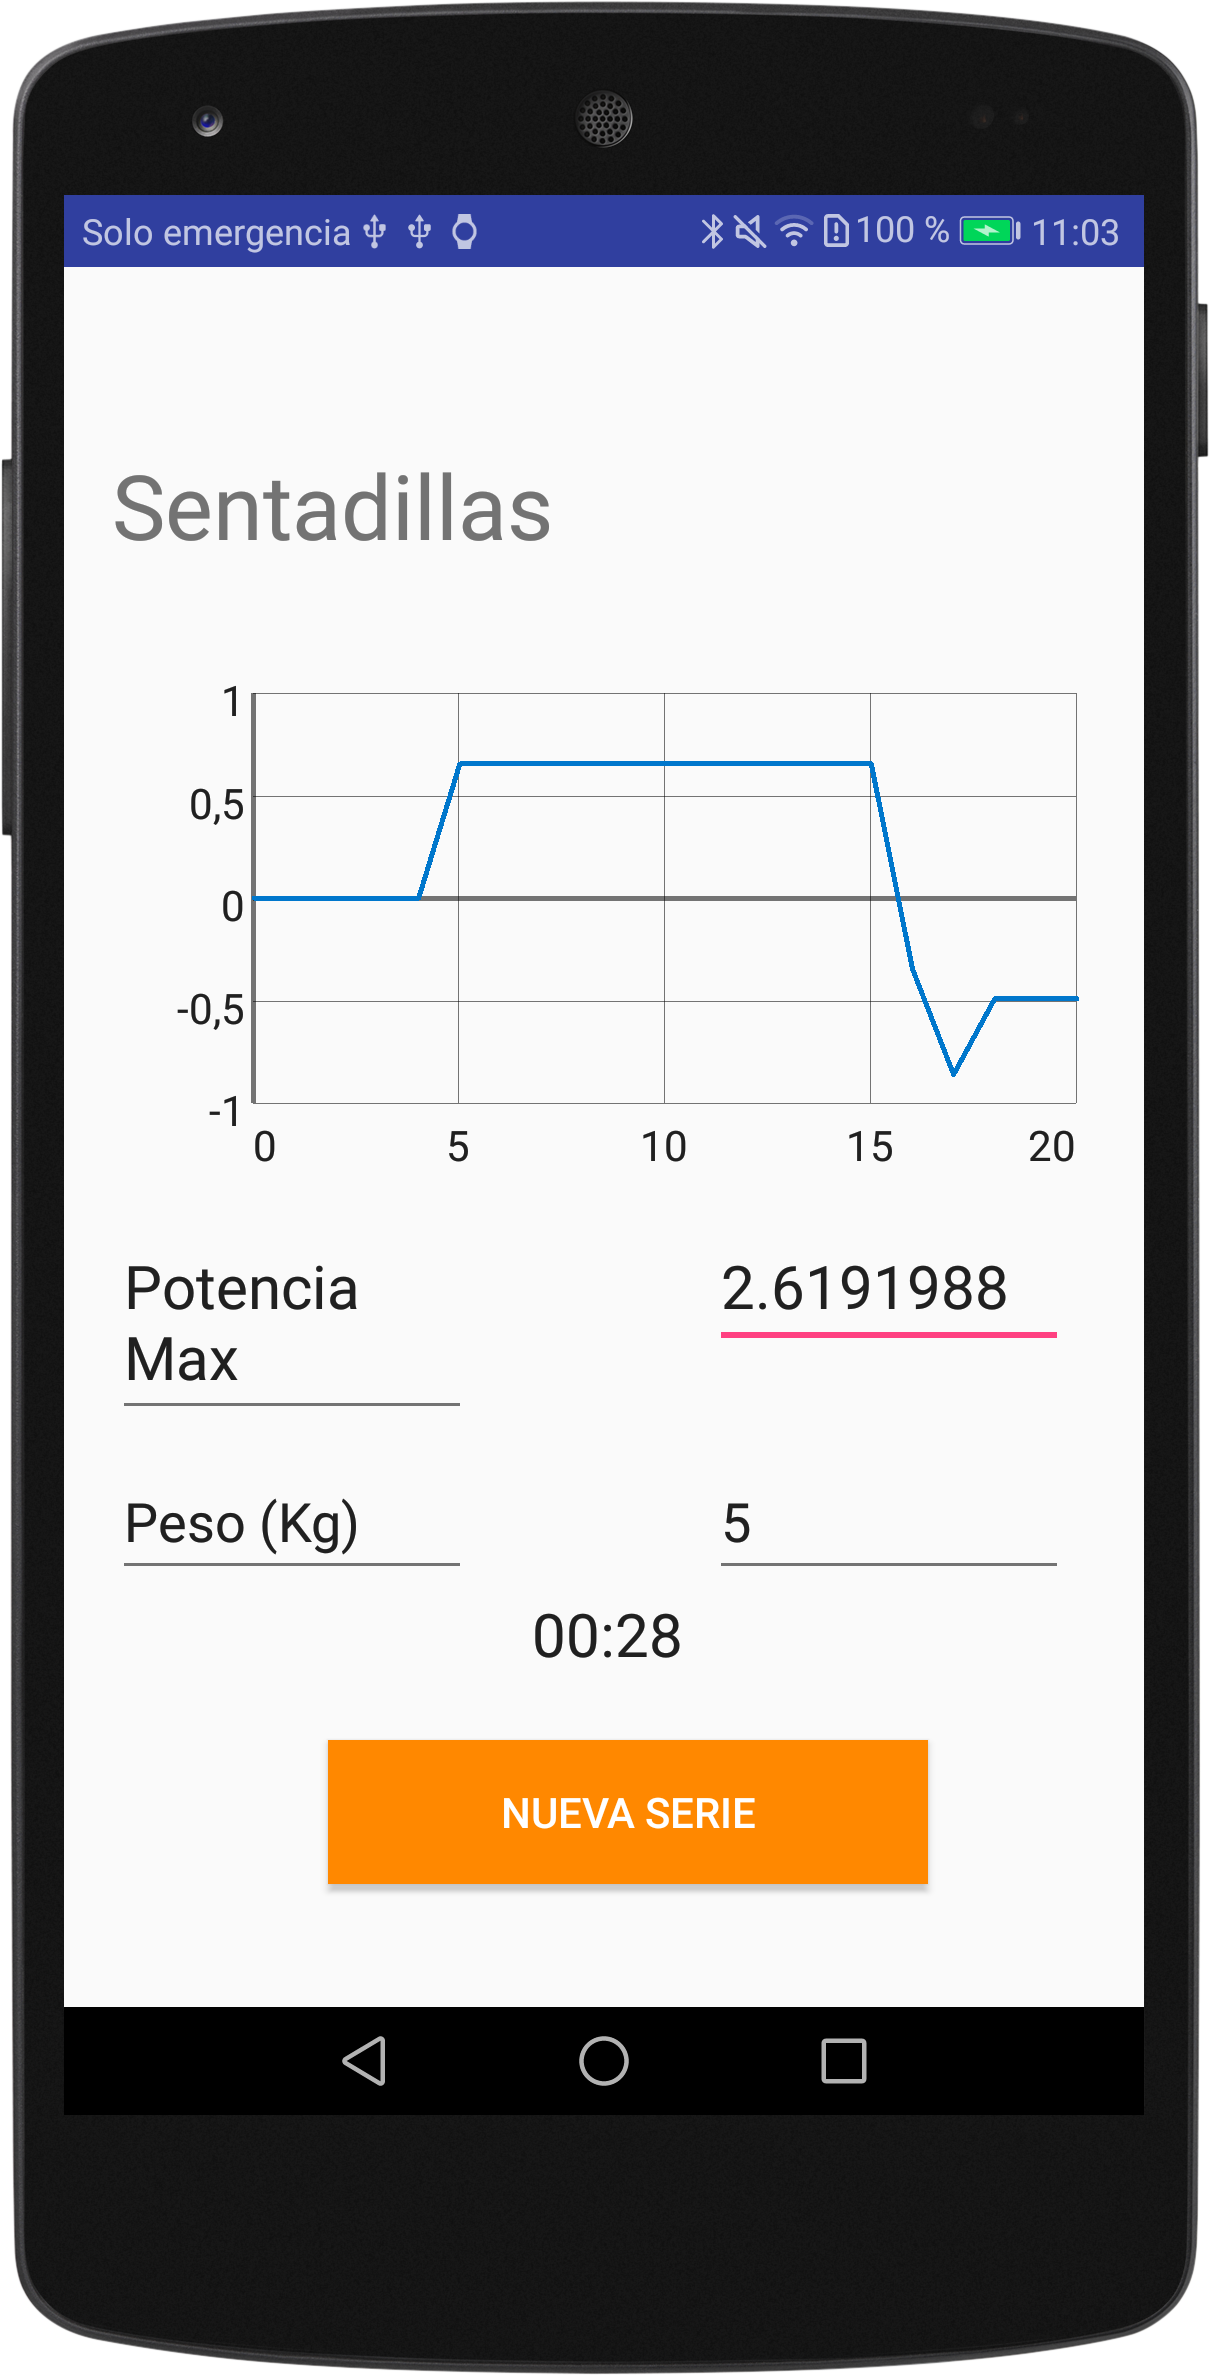
\includegraphics[scale=0.10]{imagenes/m7.png}
	\caption{Ejemplo realización ejercicio móvil}
	\label{Realización ejercicio 7}
\end{figure}

\section{Consulta del histórico}

Para realizar una consulta simplemente se debe que seleccionar en el menú de navegación la pestaña histórico y seleccionar un día del calendario.

\begin{figure}[H]
	\centering
	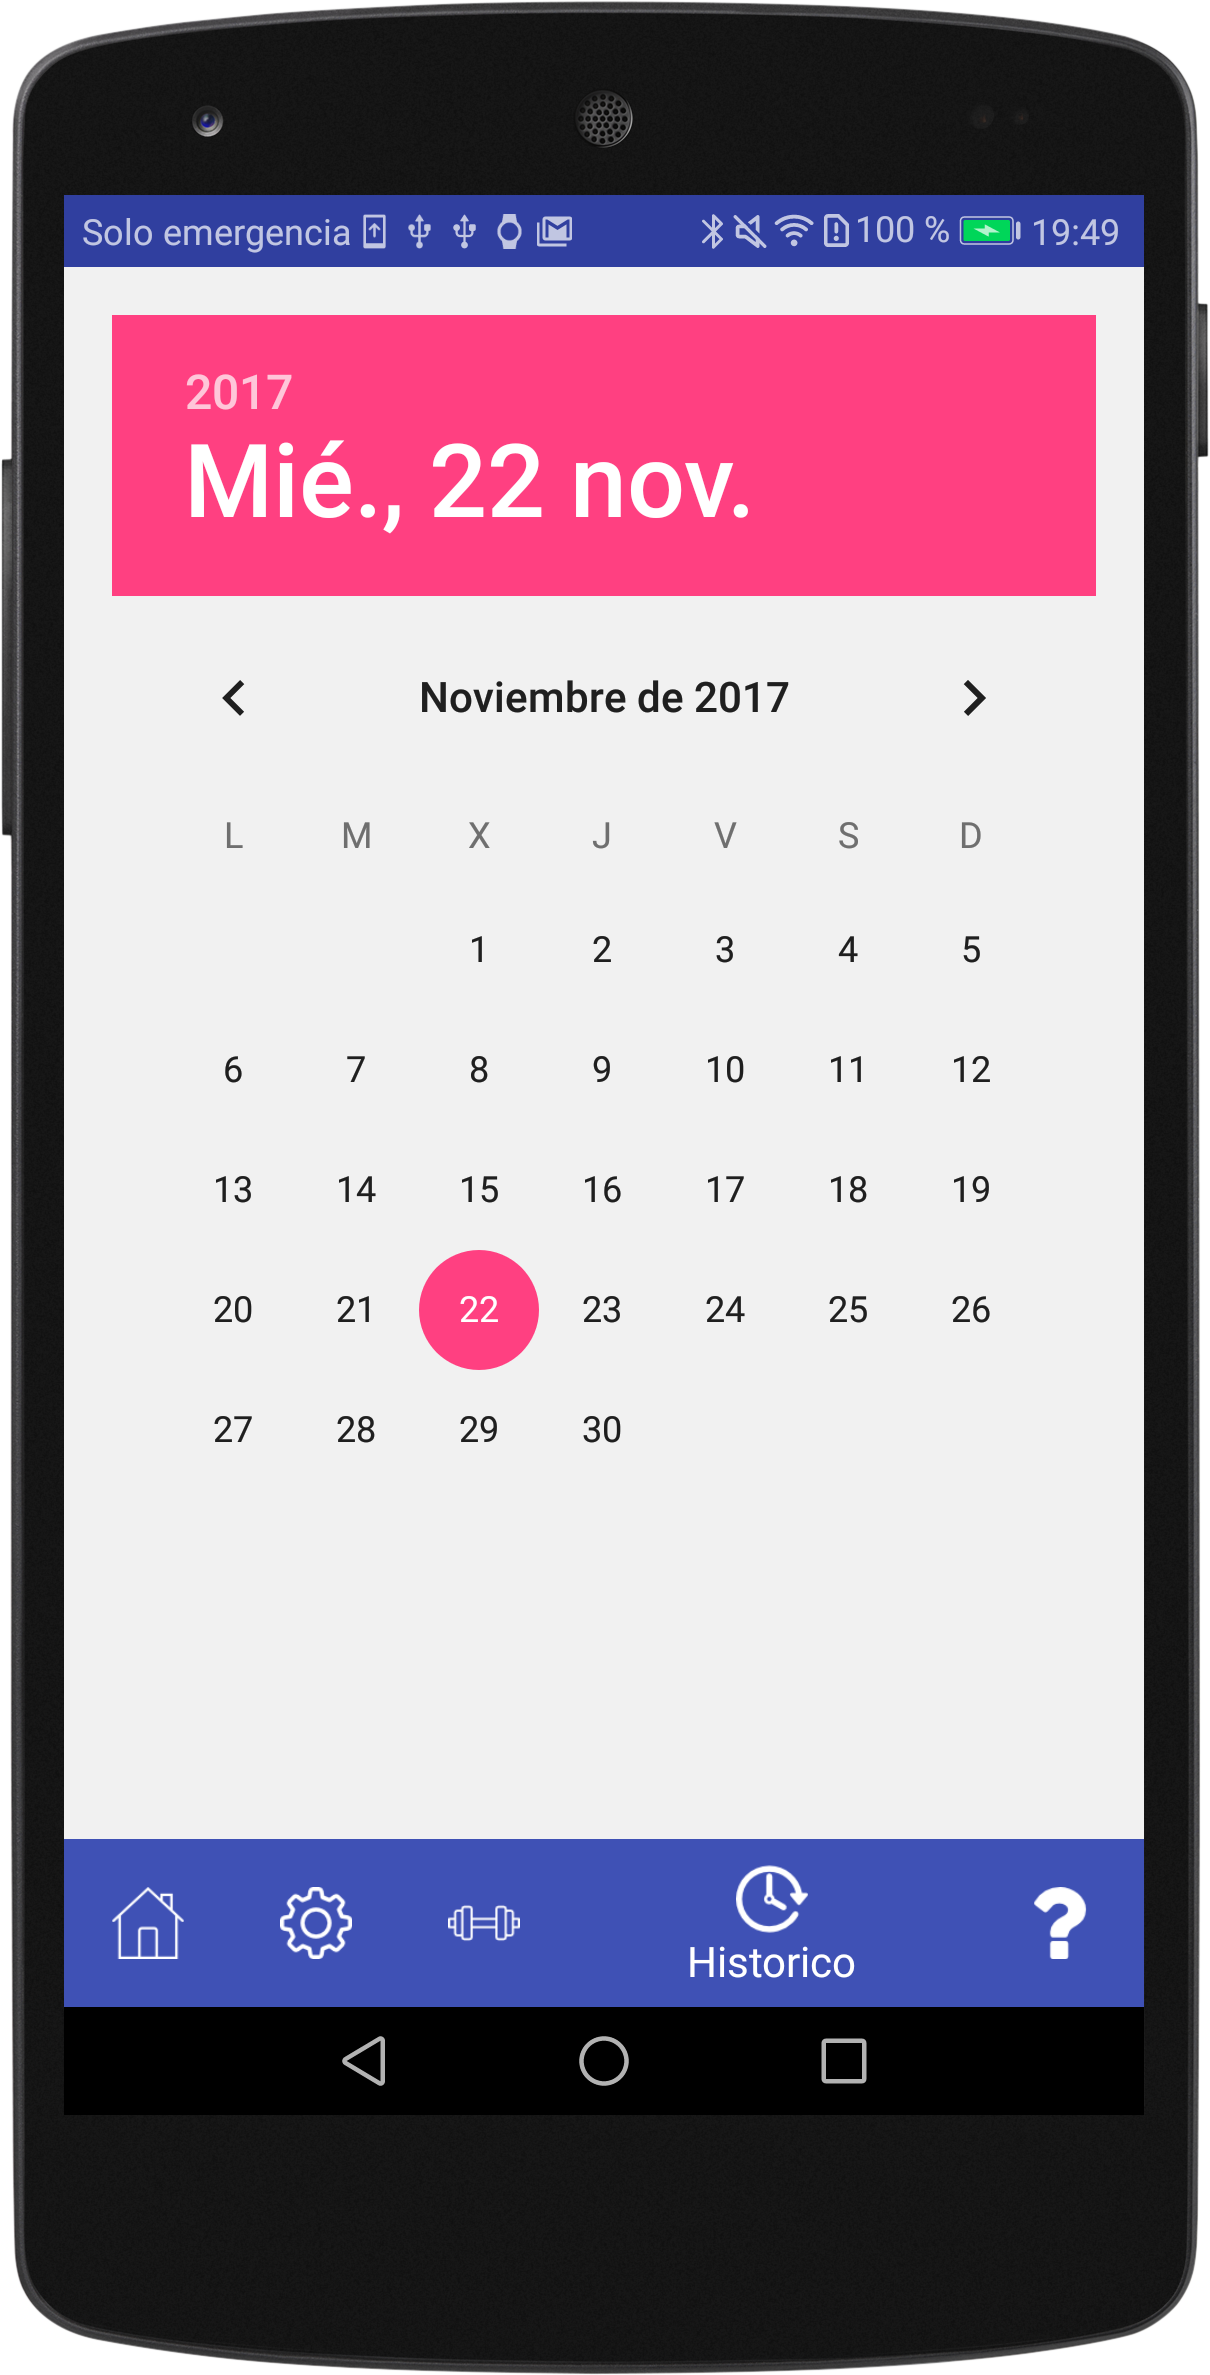
\includegraphics[scale=0.10]{imagenes/histori.png}
	\caption{Consulta del histórico}
	\label{Consulta del histórico}
\end{figure}
